\documentclass[12pt]{article}
\usepackage{amsmath}
\usepackage{graphicx}
\usepackage{hyperref}
\usepackage{listings}
\usepackage{color}

\title{Operating System Course Report - First Half of the Semester}
\author{B class}
\date{\today}

\begin{document}

\maketitle
\newpage

\tableofcontents
\newpage

\section{Introduction}
This report summarizes the topics covered during the first half of the Operating System course. It includes theoretical concepts, practical implementations, and assignments. The course focuses on the fundamentals of operating systems, including system architecture, process management, CPU scheduling, and deadlock handling.

\section{Course Overview}
\subsection{Objectives}
The main objectives of this course are:
\begin{itemize}
    \item To understand the basic components and architecture of a computer system.
    \item To learn process management, scheduling, and inter-process communication.
    \item To explore file systems, input/output management, and virtualization.
    \item To study the prevention and handling of deadlocks in operating systems.
\end{itemize}

\subsection{Course Structure}
The course is divided into two halves. This report focuses on the first half, which covers:
\begin{itemize}
    \item Basic Concepts and Components of Computer Systems
    \item System Performance and Metrics
    \item System Architecture of Computer Systems
    \item Process Description and Control
    \item Scheduling Algorithms
    \item Process Creation and Termination
    \item Introduction to Threads
    \item File Systems
    \item Input and Output Management
    \item Deadlock Introduction and Prevention
    \item User Interface Management
    \item Virtualization in Operating Systems
\end{itemize}

\section{Topics Covered}

\subsection{Basic Concepts and Components of Computer Systems}
This section explains the fundamental components that make up a computer system, including the CPU, memory, storage, and input/output devices.

\subsection{System Performance and Metrics}
This section introduces various system performance metrics used to measure the efficiency of a computer system, including throughput, response time, and utilization.

\subsection{System Architecture of Computer Systems}
Describes the architecture of modern computer systems, focusing on the interaction between hardware and the operating system.

\subsection{Process Description and Control}
Processes are a central concept in operating systems. This section covers:
\begin{itemize}
    \item Process states and state transitions
    \item Process control block (PCB)
    \item Context switching
\end{itemize}

\subsection{Scheduling Algorithms}
This section covers:
\begin{itemize}
    \item First-Come, First-Served (FCFS)
    \item Shortest Job Next (SJN)
    \item Round Robin (RR)
\end{itemize}
It explains how these algorithms are used to allocate CPU time to processes.

\subsection{Process Creation and Termination}
Details how processes are created and terminated by the operating system, including:
\begin{itemize}
    \item Process spawning
    \item Process termination conditions
\end{itemize}

\subsection{Introduction to Threads}
This section introduces the concept of threads and their relation to processes, covering:
\begin{itemize}
    \item Single-threaded vs. multi-threaded processes
    \item Benefits of multithreading
\end{itemize}

\subsection{File Systems}
File systems provide a way for the operating system to store, retrieve, and manage data. This section explains:
\begin{itemize}
    \item File system structure
    \item File access methods
    \item Directory management
\end{itemize}

\subsection{Input and Output Management}
Input and output management is key for handling the interaction between the system and external devices. This section includes:
\begin{itemize}
    \item Device drivers
    \item I/O scheduling
\end{itemize}

\subsection{Deadlock Introduction and Prevention}
Explores the concept of deadlocks and methods for preventing them:
\begin{itemize}
    \item Deadlock conditions
    \item Deadlock prevention techniques
\end{itemize}

\subsection{User Interface Management}
This section discusses the role of the operating system in managing the user interface. Topics covered include:
\begin{itemize}
    \item Graphical User Interface (GUI)
    \item Command-Line Interface (CLI)
    \item Interaction between the user and the operating system
\end{itemize}

\subsection{Virtualization in Operating Systems}
Virtualization allows multiple operating systems to run concurrently on a single physical machine. This section explores:
\subsubsection{Hypervisor dan Virtual Machines}
\begin{enumerate}
    \item \textbf{Hypervisor}
    \newline Hypervisor adalah perangkat lunak yang memungkinkan beberapa sistem operasi berjalan pada satu perangkat keras fisik. Salah satu manfaat utama dari penggunaan hypervisor adalah kemampuannya untuk memigrasikan mesin virtual antar sistem tanpa gangguan yang signifikan bagi pengguna. Sebagai contoh, dalam kasus insiden perangkat keras, mesin virtual dapat dipindahkan ke sistem lain dengan sangat sedikit usaha. Dalam kondisi terbaik, pengguna bahkan mungkin tidak menyadari bahwa telah terjadi migrasi \cite{satra2023}. Tanpa hypervisor, setiap sistem operasi akan mencoba mengakses perangkat keras secara langsung, yang dapat menyebabkan konflik dan ketidakstabilan. Dengan hypervisor, semua akses ke perangkat keras dimediasi dengan aman, sehingga memungkinkan lebih dari satu mesin virtual untuk berbagi sumber daya yang sama \cite{portnoy2012}. Hypervisor memisahkan perangkat keras dari sistem operasi, memungkinkan kontrol yang lebih baik atas sumber daya. Berdasarkan cara hypervisor dijalankan, terdapat 2 tipe atau jenis dari hypervisor yang dapat dilihat sebagai berikut:
    \begin{itemize}
        \item \textbf{Bare-metal Hypervisor}
        \begin{figure}[h]
            \centering
            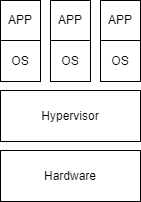
\includegraphics[width=0.3\textwidth]{asset/hypervisor_tipe_1.png}
            \caption{Ilustrasi Bare-metal Hypervisor}
        \end{figure}
        Bare-metal Hypervisor (juga dikenal sebagai hypervisor tipe 1) berjalan langsung di atas perangkat keras tanpa memerlukan sistem operasi host. Ini memberikan kinerja yang lebih tinggi karena tidak ada lapisan tambahan antara perangkat keras dan hypervisor. VMware ESXi dan Microsoft Hyper-V adalah contoh populer dari jenis hypervisor ini, sering digunakan dalam lingkungan server di mana efisiensi dan stabilitas menjadi prioritas utama \cite{satra2023}. Bare-metal hypervisor ini sangat ideal untuk aplikasi yang memerlukan sumber daya tinggi dan latensi rendah.

        \item \textbf{Hosted Hypervisor}
        \begin{figure}[h]
            \centering
            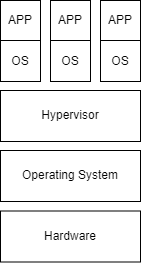
\includegraphics[width=0.3\textwidth]{asset/hypervisor_tipe_2.png}
            \caption{Ilustrasi Hosted Hypervisor}
        \end{figure}
        Hosted hypervisor (atau hypervisor tipe 2) berjalan di atas sistem operasi host, yang menyediakan fleksibilitas lebih tetapi dengan potensi penurunan kinerja dibandingkan dengan bare-metal hypervisor. Contoh dari hosted hypervisor adalah VMware Workstation dan Oracle VirtualBox, yang sering digunakan untuk lingkungan pengembangan atau uji coba \cite{portnoy2012}. Hosted hypervisor lebih mudah diatur dan lebih user-friendly, namun karena berjalan di atas sistem operasi, ada lapisan tambahan yang memperlambat akses ke perangkat keras.
    \end{itemize}
    \item \textbf{Virtual Machines}
    \newline Mesin virtual (VM) adalah representasi virtual dari perangkat keras komputer fisik. Setiap mesin virtual beroperasi seperti komputer independen, dengan sumber daya virtual seperti CPU, memori, penyimpanan, dan kartu jaringan, yang diatur oleh hypervisor. Dalam lingkungan ini, VM dapat menjalankan berbagai sistem operasi secara bersamaan di atas satu perangkat keras fisik. Hal ini memungkinkan perusahaan untuk mengkonsolidasikan infrastruktur mereka, mengurangi biaya perangkat keras, dan meningkatkan efisiensi operasional \cite{portnoy2012}. 
    \begin{figure}[h]
        \centering
        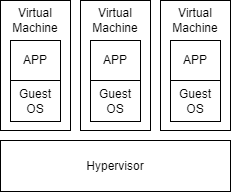
\includegraphics[width=0.3\textwidth]{asset/virtual_machine.png}
        \caption{Ilustrasi Virtual Machine}
    \end{figure}
    Penggunaan mesin virtual juga memungkinkan fleksibilitas dalam pengelolaan, seperti kemampuan untuk mengkloning, menghentikan sementara, atau menghapus VM tanpa mengganggu sistem lain yang berjalan pada perangkat keras yang sama. Ini sangat berguna dalam lingkungan pengembangan dan produksi di mana perubahan cepat dan skalabilitas dibutuhkan \cite{satra2023}.
\end{enumerate}

\subsubsection{Contoh Penerapan Virtualisasi pada Sistem Operasi}
\begin{enumerate}
    \item \textbf{VMWare} \\
    VMWare adalah salah satu solusi virtualisasi paling populer yang digunakan secara luas di berbagai industri. VMWare menyediakan platform virtualisasi berbasis hypervisor yang memungkinkan pengguna untuk membuat dan mengelola mesin virtual (VM) di atas perangkat keras fisik tanpa perlu menginstal sistem operasi host. Dengan teknologi VMWare vSphere, perusahaan dapat menjalankan beberapa VM di atas satu perangkat keras fisik, yang menghasilkan efisiensi yang lebih tinggi dalam penggunaan sumber daya serta pengurangan biaya infrastruktur. Salah satu keunggulan VMWare adalah stabilitasnya yang tinggi dan fitur-fitur enterprise-grade seperti vMotion yang memungkinkan migrasi VM tanpa downtime.

    VMWare memiliki beberapa produk virtualisasi, di antaranya VMWare Workstation yang ditujukan untuk lingkungan desktop, dan VMWare ESXi yang ditujukan untuk lingkungan server. VMWare juga mendukung virtualisasi jaringan melalui produk NSX dan memiliki integrasi kuat dengan layanan cloud. Kemampuan untuk mengelola infrastruktur virtual secara terpusat melalui VMWare vCenter memudahkan administrasi dan pengawasan, membuat VMWare menjadi solusi pilihan bagi perusahaan yang memerlukan solusi virtualisasi tingkat lanjut.

    \item \textbf{VirtualBox} \\
    VirtualBox adalah perangkat lunak virtualisasi open-source yang dikembangkan oleh Oracle. Berbeda dengan VMWare yang lebih banyak digunakan dalam lingkungan enterprise, VirtualBox lebih populer di kalangan pengguna individu atau pengembang yang membutuhkan lingkungan uji coba yang fleksibel dan mudah diatur. VirtualBox memungkinkan pengguna untuk menjalankan berbagai sistem operasi di dalam satu perangkat keras, baik itu Windows, Linux, macOS, atau sistem operasi lainnya, dalam bentuk mesin virtual. Kelebihan utama VirtualBox adalah sifatnya yang gratis dan mudah digunakan, serta dukungan untuk berbagai platform dan arsitektur perangkat keras.

    Meskipun lebih cocok untuk pengguna desktop atau pengembang, VirtualBox juga memiliki beberapa fitur tingkat lanjut seperti snapshot, yang memungkinkan pengguna untuk menyimpan kondisi mesin virtual pada titik tertentu dan kembali ke kondisi tersebut jika diperlukan. Selain itu, VirtualBox mendukung fitur shared folders dan clipboard antara sistem host dan guest, membuat proses transfer data antar sistem lebih efisien. Karena keunggulan fleksibilitas dan kemudahannya, VirtualBox sering digunakan oleh pengembang untuk menguji perangkat lunak di berbagai lingkungan sistem operasi tanpa perlu mengatur perangkat keras tambahan.

    \item \textbf{Kernel-Based Virtual Machine (KVM)} \\
    Kernel-Based Virtual Machine (KVM) adalah solusi virtualisasi berbasis kernel untuk sistem operasi Linux. KVM memungkinkan Linux untuk berfungsi sebagai hypervisor, dengan setiap instance VM berjalan sebagai proses dalam sistem host, namun dengan isolasi yang kuat. KVM memanfaatkan arsitektur x86 dengan ekstensi virtualisasi (Intel VT atau AMD-V) untuk menjalankan VM dengan kinerja yang mendekati perangkat keras fisik. KVM sering digunakan dalam lingkungan server yang memerlukan efisiensi dan kontrol penuh atas infrastruktur virtual.

    Salah satu keunggulan KVM adalah integrasinya yang dalam dengan kernel Linux, memungkinkan kinerja yang optimal dan penggunaan sumber daya yang lebih efisien. Selain itu, KVM adalah pilihan utama dalam banyak lingkungan cloud, termasuk OpenStack, yang memanfaatkan KVM untuk mengelola mesin virtual. Dengan kombinasi antara kinerja, skalabilitas, dan dukungan komunitas open-source yang besar, KVM menjadi pilihan populer bagi banyak perusahaan yang mengandalkan infrastruktur virtual berbasis Linux.

    \item \textbf{Docker} \\
    Docker adalah platform yang berbeda dari solusi hypervisor tradisional karena menggunakan pendekatan containerization alih-alih virtualisasi penuh. Alih-alih membuat mesin virtual yang sepenuhnya terisolasi, Docker menjalankan aplikasi dalam kontainer yang berbagi kernel dengan sistem host, tetapi tetap terisolasi pada tingkat sistem file, proses, dan jaringan. Ini memungkinkan aplikasi untuk berjalan di lingkungan terisolasi tanpa memerlukan hypervisor atau virtualisasi perangkat keras. Docker memberikan keuntungan dalam hal kecepatan dan efisiensi dibandingkan dengan VM tradisional, karena kontainer lebih ringan dan dapat di-deploy dengan lebih cepat.

    Docker sangat populer di kalangan pengembang dan tim DevOps karena kemampuannya untuk membuat aplikasi yang dapat di-deploy dengan konsisten di berbagai lingkungan, baik di lokal pengembang, server uji coba, maupun di cloud. Dengan Docker, pengembang dapat membungkus aplikasi beserta seluruh dependensinya dalam sebuah kontainer yang kemudian dapat dijalankan di mana saja. Keuntungan ini mempermudah kolaborasi dan pengelolaan aplikasi, terutama dalam lingkungan pengembangan modern yang membutuhkan fleksibilitas dan portabilitas.
\end{enumerate}

\section{Assignments and Practical Work}
\subsection{Assignment 1: Process Scheduling}
Students were tasked with implementing various process scheduling algorithms (e.g., FCFS, SJN, and RR) and comparing their performance under different conditions.

\subsection{Assignment 2: Deadlock Handling}
In this assignment, students were asked to simulate different deadlock scenarios and explore various prevention methods.
Pertanyaan:
Simulasikan skenario deadlock yang melibatkan empat proses dan empat sumber daya. Kemudian, terapkan dan demonstrasikan tiga metode pencegahan deadlock: Mutual Exclusion, Hold and Wait, dan Circular Wait.

\begin{python}
    import threading
    import time

    # Sumber Daya
    R1 = threading.Lock()
    R2 = threading.Lock()
    R3 = threading.Lock()
    R4 = threading.Lock()

    # Simulasi Deadlock
    def proses_1():
        R1.acquire()
        time.sleep(1)
        R2.acquire()
        time.sleep(1)
        R3.acquire()
        time.sleep(1)
        R4.acquire()
        R4.release()
        R3.release()
        R2.release()
        R1.release()

    def proses_2():
        R2.acquire()
        time.sleep(1)
        R3.acquire()
        time.sleep(1)
        R4.acquire()
        time.sleep(1)
        R1.acquire()
        R1.release()
        R4.release()
        R3.release()
        R2.release()

    def proses_3():
        R3.acquire()
        time.sleep(1)
        R4.acquire()
        time.sleep(1)
        R1.acquire()
        time.sleep(1)
        R2.acquire()
        R2.release()
        R1.release()
        R4.release()
        R3.release()

    def proses_4():
        R4.acquire()
        time.sleep(1)
        R1.acquire()
        time.sleep(1)
        R2.acquire()
        time.sleep(1)
        R3.acquire()
        R3.release()
        R2.release()
        R1.release()
        R4.release()

    # Menjalankan semua proses
    p1 = threading.Thread(target=proses_1)
    p2 = threading.Thread(target=proses_2)
    p3 = threading.Thread(target=proses_3)
    p4 = threading.Thread(target=proses_4)

    p1.start()
    p2.start()
    p3.start()
    p4.start()

    p1.join()
    p2.join()
    p3.join()
    p4.join()

    print("Simulasi deadlock selesai.")

    # Metode pencegahan deadlock dapat diimplementasikan dan diuji dengan cara serupa

\end{python}

\subsection{Assignment 3: Multithreading and Amdahl's Law}
This assignment involved designing a multithreading scenario to solve a computationally intensive problem. Students then applied **Amdahl's Law** to calculate the theoretical speedup of the program as the number of threads increased.

\subsection{Assignment 4: Simple Command-Line Interface (CLI) for User Interface Management}
Students were tasked with creating a simple **CLI** for user interface management. The CLI should support basic commands such as file manipulation (creating, listing, and deleting files), process management, and system status reporting.

\subsection{Assignment 5: File System Access}
In this assignment, students implemented file system access routines, including:
\begin{itemize}
    \item File creation and deletion
    \item Reading from and writing to files
    \item Navigating directories and managing file permissions
\end{itemize}

\section{Conclusion}
Virtualisasi sistem operasi menawarkan berbagai manfaat signifikan untuk pengelolaan sumber daya komputer. Dengan memungkinkan beberapa sistem operasi berjalan secara bersamaan pada satu mesin fisik, virtualisasi meningkatkan efisiensi penggunaan hardware, menurunkan biaya operasional, dan memberikan fleksibilitas tinggi dalam menjalankan berbagai aplikasi. Teknologi seperti hypervisor memungkinkan pemisahan total antara sistem operasi dan perangkat keras fisik, sehingga memungkinkan isolasi dan pengelolaan sumber daya yang lebih baik. Sebagai hasilnya, pengguna dapat menjalankan beberapa lingkungan komputasi yang terisolasi dengan aman pada satu platform fisik.
Namun, ada juga beberapa kekurangan yang perlu dipertimbangkan, seperti kompleksitas yang lebih tinggi dalam pengelolaan dan potensi risiko keamanan. Ketergantungan pada hypervisor juga dapat menjadi titik lemah jika terjadi kerentanan atau serangan pada lapisan tersebut. Meskipun begitu, dengan pemahaman yang baik dan manajemen yang tepat, virtualisasi tetap menjadi solusi yang kuat dan fleksibel dalam pengelolaan infrastruktur TI. Kombinasi antara keuntungan ekonomi dan fleksibilitas operasional menjadikan virtualisasi sebagai pilihan utama dalam banyak organisasi modern.

\begin{thebibliography}
    \bibitem[1]{satra2023} Satra, R., Syafie, L., & Tubagus, M. (2023, May). Comparison of server technologies using Kernel-based virtual machine and container virtualization. In AIP Conference Proceedings (Vol. 2595, No. 1). AIP Publishing.
    \bibitem[2]{portnoy2012} Portnoy, M. (2012). Virtualization essentials (Vol. 19). John Wiley & Sons.
\end{thebibliography}
\end{document}